\section{Extraction des paramètres}

Une fois la qualité des mesures évaluée, il s'agit maintenant d'en extraire les paramètres nécessaires à la fois à la synthèse par FRF et à la synthèse modale.

\subsection{Paramètres de synthèse FRF}

Dans le cadre de la première, l'admittance $Y_{body}$ du corps sans corde de l'instrument est obtenue de façon directe au travers des mesures de la partie précédente : ne restent à être extraites uniquement les valeurs des fréquences de résonance de la corde et celles de leurs amortissements.\\

Pour ce faire, et en se basant sur la relation [REF NEEDED], il est en théorie possible de commencer par extraire $Y_{string}$ des valeurs mesurées de $Y_{body}$ et $Y_{total}$ puis d'analyser $Y_{string}$ et d'identifier au moyen de la relation [REF NEEDED] les fréquences et amortissements. Malheureusement il existe entre l'admittance de corde et les deux autres une différence d'ordre de grandeur telle que les simple bruit de mesure de ces dernières noie le signal qui aurait du être $Y_{string}$ : cela nous pousse donc à la mesurer directement sur banc de corde, ce qui par manque de temps ne sera pas fait au cours de ce projet. La suite de cette partie s'attache cependant à mettre en place un protocole d'extraction des fréquences et amortissement en supposant la connaissance de $Y_{string}$.\\

\subsubsection{Analyse ESPRIT par bandes}

Supposons donc que nous disposions d'une admittance $Y$, issue d'une mesure sur corde : il est donc à priori possible, en extrayant sa fréquence fondamentale via produit spectral, puis en recherchant chaque harmonique sur une plage de fréquence dictée par les valeurs des harmoniques précédents, d'obtenir une première série de valeurs de fréquences de modes. Cette méthode n'a cependant pas le mérite d'être très précise, et ne renvoie pas non plus de valeurs d'amortissement : elle peut cependant servir de base à une analyse par méthode à haute-résolution (dans le cas présent, la méthode ESPRIT [REF NEEDED]) centrée autour de ces premières approximations de fréquences.\\
Le signal est dans un premier temps filtré autour de chacun de ces harmoniques par filtre passe-bande à réponse finie et phase linéaire, ceci afin de garantir des signaux filtrés présentant les mêmes pôles que le signal d'origine (le résultat est visible en [REF NEEDED]). Afin d'accélérer l'analyse par méthode ESPRIT, il est ensuite modulé par la fréquences de l'harmonique approximatif afin de la recentrer autour de $0 Hz$ (voir [REF NEEDED]) et de permettre une décimation (voir [REF NEEDED]). S'ensuit alors une analyse par ESPRIT, qui donne directement accès aux valeurs exactes de fréquences propres et amortissement de $Y$.

\begin{figure}[h]
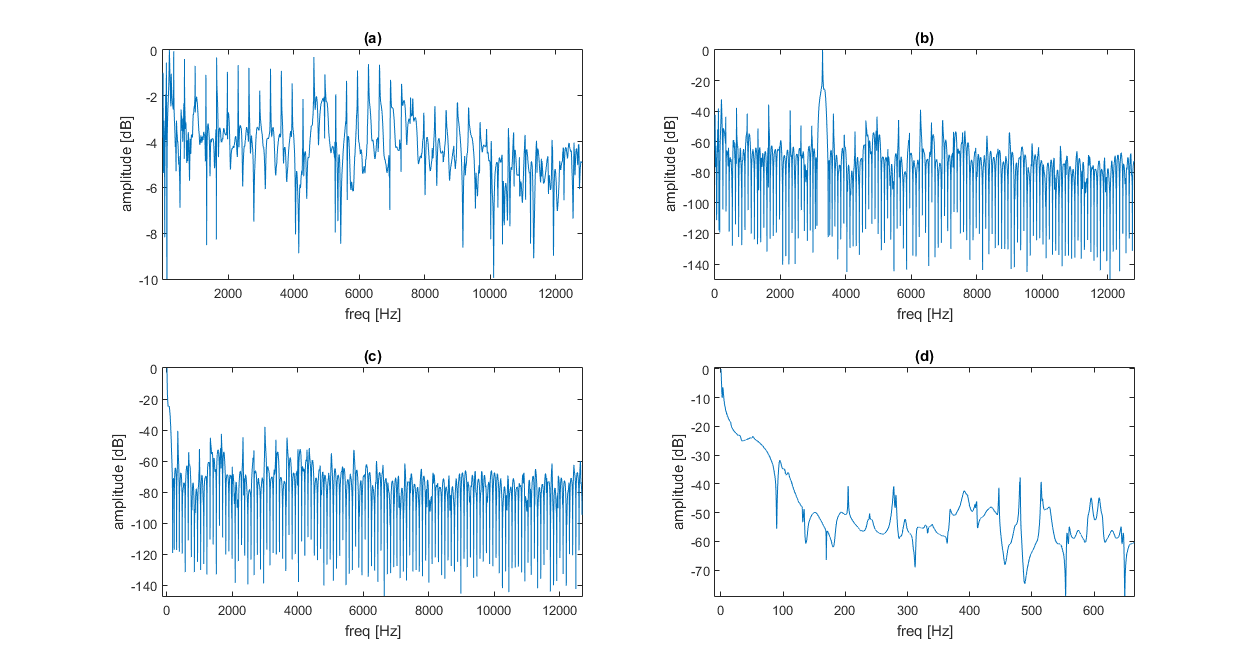
\includegraphics[scale=0.5]{figures/pre_proc.png}
\caption{\textit{(a) spectre du signal d'entrée - (b) spectre du signal filtré sur un harmonique - (c) spectre du signal modulé par la fréquence de l'harmonique - (d)spectre du signal décimé.}}
\label{pre_proc}
\end{figure}

\subsubsection{Valeurs utilisées}

A défaut d'utiliser ce protocole pour extraire les paramètres de la synthèse par FRF, les valeurs fournies par Woodhouse [REF NEEDED] seront utilisées.

\subsection{Paramètres de synthèse modale}

Les paramètres utilisés en entré de la synthèse modale sont des paramètres physiques, notamment : [THEIS ?]. N'ayant pu les mesurer pour la plupart, nous utiliserons des valeurs...
\\\\

Les paramètres ayant été rassemblés, il est maintenant possible de produire par chacune des méthodes de synthèses 

\section{Paramètres de synthèse modale}


